% 15.3 AREA
% TWO SIDEWAYS PARABOLAS
\ifnum \Version=1  
    \part The area of the region bounded by $x=y^2-1$ and $x=2y^2 - 2$ is $\displaystyle  \int_a^b \int_c^d f(x,y) \, dx \, dy$,  where $a=\framebox{\strut\hspace{1cm}}$, $b=\framebox{\strut\hspace{1cm}}$, $c=\framebox{\strut\hspace{2cm}}$, $d=\framebox{\strut\hspace{2cm}}$, and $f(x,y) = \framebox{\strut\hspace{2cm}}$.
    
    \ifnum \Solutions=1 
    {\color{DarkBlue} We want to determine where the two curves intersect. Setting them equal to each other: 
    \begin{align}
        y^2-1 &= 2y^2 - 2 \\
        1 &= y^2 \\
        y &= \pm 1
    \end{align}
    To obtain the $x-$coordinates, we can use either curve. Substituting the two $y-$values into either curve gives us two intersection points
    $$(0,-1), (0,+1)$$
    It can help to sketch the two curves, as shown in the diagram below. 
       \begin{center}     
    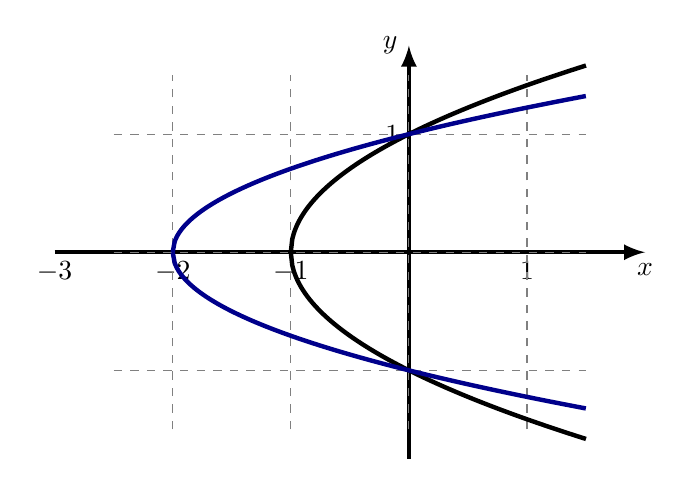
\begin{tikzpicture}[scale=1.5]
      \draw[ultra thick,->,>=latex] (-3,0)--(2,0) node[below] {$x$};
      \draw[ultra thick,->,>=latex] (0,-1.75)--(0,1.75) node[left] {$y$};
      \draw (0,1) node[left] {$1$};  
      \draw (-1,0) node[below] {$-1$};          
      \draw (-2,0) node[below] {$-2$};          
      \draw (-3,0) node[below] {$-3$};          
      \draw (1,0) node[below] {$1$};
      \draw[help lines,gray,thin,dashed] (-2.5, -1.5) grid (1.5, 1.5);
      \draw[domain=-1:1.5,ultra thick,samples=200] plot ({\x},{sqrt(\x + 1))});
      \draw[domain=-1:1.5,ultra thick,samples=200] plot ({\x},{-sqrt(\x + 1))});
      \draw[domain=-2:1.5,ultra thick,DarkBlue,samples=200] plot ({\x},{sqrt(\x/2 + 1))});
      \draw[domain=-2:1.5,ultra thick,DarkBlue,samples=200] plot ({\x},{-sqrt(\x/2 + 1))});      
    \end{tikzpicture}
    \end{center}     
    The region is bounded on the \textbf{left} by $x=2y^2-2$, and bounded on the \textbf{right} by $x=y^2-1$. The region is 
    $$R = \{(x,y) \in \mathbb R^2 \, | \, -1\le y \le 1, \quad 2y^2-2 < x < y^2-1\}$$
    Therefore, 
    \begin{align}
        a & = -1 \\
        b &= +1 \\
        c &= 2y^2 -2 \\
        d &= y^2-1 \\
        f &= 1
    \end{align}
    }
   \else

   \fi
\fi 







% AVERAGE VALUE AND TRIANGULAR REGION
\ifnum \Version=2
    \part The average value of $f(x,y) = 12-8xy$ over the region in the first quadrant bounded by $x=0$, $y=0$, and $y=4-2x$ is $\displaystyle  \int_a^b \int_c^d g(x,y) \, dx \, dy$,  where $a=\framebox{\strut\hspace{1cm}}$, $b=\framebox{\strut\hspace{1cm}}$, $c=\framebox{\strut\hspace{2cm}}$, $d=\framebox{\strut\hspace{2cm}}$, and $g(x,y) = \framebox{\strut\hspace{2cm}}$.

    \ifnum \Solutions=1 
    {\color{DarkBlue} 
    The average value of a function $f(x,y)$ over a region $R$ is given by 
    \begin{align}
        \text{Average value of }f\text{ over region }R &= \frac{1}{\text{area of region }R}\iint_R f \, dA \\&= \iint_R \frac{f(x,y)}{\text{area of region }R} \, dA
    \end{align}
    Therefore to obtain $g(x,y)$ we can calculate
    \begin{align}
        g(x,y) = \frac{f(x,y)}{\text{area of region }R}
    \end{align}
    So we need the area of the region. It can help to sketch the region, as shown in the diagram below. 
       \begin{center}     
        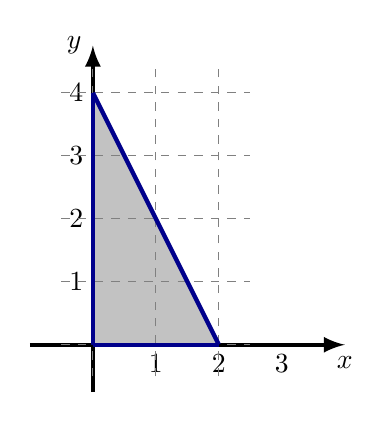
\begin{tikzpicture}[scale=0.8]
        \draw[fill=gray!80!black, opacity=0.4] (0,0) -- (0,4) -- (2,0);        
        \draw[ultra thick,->,>=latex] (-1,0)--(4,0) node[below] {$x$};
        \draw[ultra thick,->,>=latex] (0,-0.75)--(0,4.75) node[left] {$y$};
        \draw (1,0) node[below] {$1$};          
        \draw (2,0) node[below] {$2$};          
        \draw (3,0) node[below] {$3$};          
        \draw (0,1) node[left] {$1$};        
        \draw (0,2) node[left] {$2$};
        \draw (0,3) node[left] {$3$};
        \draw (0,4) node[left] {$4$};
        \draw[help lines,gray,thin,dashed] (-0.5, -0.5) grid (2.5, 4.5);
        \draw[domain=0:2,ultra thick,DarkBlue,samples=200] plot ({\x},{4-2*\x });
        \draw[domain=0:2,ultra thick,DarkBlue,samples=200] plot ({\x},{0 });
        \draw[ultra thick,-,DarkBlue,>=latex] (0,0)--(0,4);
    \end{tikzpicture}
    \end{center}     
    The region is bounded on the \textbf{right} by $y=4-2x$, or $x=2-y/2$. The region is also bounded on the \textbf{left} by $x=0$. The region is 
    $$R = \{(x,y) \in \mathbb R^2 \, | \, 0\le y \le 4, \ 0 < x < 2-y/2\}$$
    The area of the region is half the area of the rectangle whose length is 2 and height is 4. 
    $$\text{area of triangular region} = \frac12 ( 2 \cdot 4) = 4$$    
    Therefore, 
    \begin{align}
        a & = 0 \\
        b &= 4 \\
        c &= 0 \\
        d &= 2-y/2 \\
        g &= \frac{12-8xy}{4} = 3 - 2xy
    \end{align}
    }
   \else

   \fi
\fi 





% SIDEWAYS PARABOLA AND A LINEAR
\ifnum \Version=3
    \part The area of the region bounded by $x=-y^2$ and $y=x+2$ is $\displaystyle  \int_a^b \int_c^d f(x,y) \, dx \, dy$,  where $a=\framebox{\strut\hspace{1cm}}$, $b=\framebox{\strut\hspace{1cm}}$, $c=\framebox{\strut\hspace{2cm}}$, $d=\framebox{\strut\hspace{2cm}}$, and $f(x,y) = \framebox{\strut\hspace{2cm}}$.
    
    \ifnum \Solutions=1 
    {\color{DarkBlue} We want to determine where the two curves intersect. Setting them equal to each other: 
    \begin{align}
        -y^2 &= y - 2 \\
        0 &= y^2 + y - 2 \\
        0 &= (y+2)(y-1) \\
        y &= -2, 1
    \end{align}
    To obtain the $x-$coordinates, we can use either curve. Substituting the two $y-$values into either curve gives us two intersection points
    $$(-4,-2), (-1,1)$$
    It can help to sketch the two curves, as shown in the diagram below. 
       \begin{center}     
    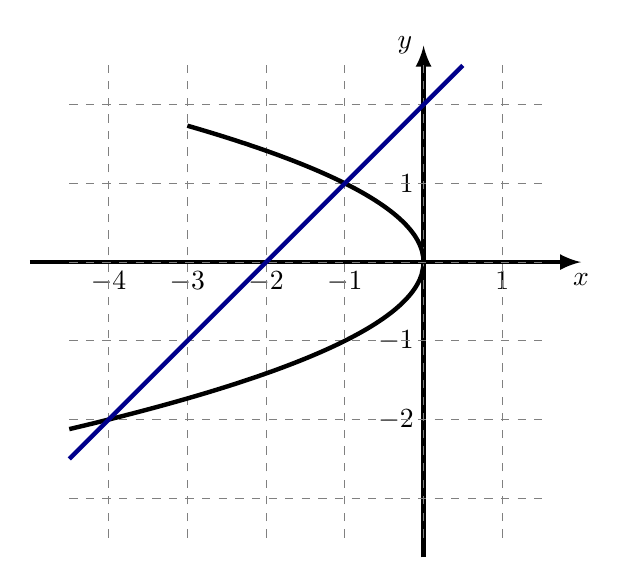
\begin{tikzpicture}[scale=1.0]
      \draw[ultra thick,->,>=latex] (-5,0)--(2,0) node[below] {$x$};
      \draw[ultra thick,->,>=latex] (0,-3.75)--(0,2.75) node[left] {$y$};
      \draw (-1,0) node[below] {$-1$};          
      \draw (-2,0) node[below] {$-2$};          
      \draw (-3,0) node[below] {$-3$};          
      \draw (-4,0) node[below] {$-4$};          
      \draw (1,0) node[below] {$1$};
      \draw (0,1) node[left] {$1$};        
      \draw (0,-1) node[left] {$-1$};
      \draw (0,-2) node[left] {$-2$};
      \draw[help lines,gray,thin,dashed] (-4.5, -3.5) grid (1.5, 2.5);
      \draw[domain=-3:0,ultra thick,samples=200] plot ({\x},{sqrt(-\x )});
      \draw[domain=-4.5:0,ultra thick,samples=200] plot ({\x},{-sqrt(-\x )});
      \draw[domain=-4.5:0.5,ultra thick,DarkBlue,samples=200] plot ({\x},{\x+2});
    \end{tikzpicture}
    \end{center}     
    The region is bounded on the \textbf{right} by $x=-y^2$, and bounded on the \textbf{left} by $x=y-2$. The region is 
    $$R = \{(x,y) \in \mathbb R^2 \, | \, -2\le y \le 1, \quad y-2 < x < -y^2\}$$
    Therefore, 
    \begin{align}
        a & = -2 \\
        b &= +1 \\
        c &= y -2 \\
        d &= -y^2 \\
        f &= 1
    \end{align}
    }
   \else

   \fi
\fi 




% AVERAGE VALUE TRIANGULAR REGION
% MESSY ALGEBRA - COULD BE SIMPLIFIED BY CHANGING F
\ifnum \Version=4
    \part The average value of $f(x,y) = 16x+20y$ over the region bounded by $x=2$, $y=4$, and $y=2-x/2$ is $\displaystyle  \int_a^b \int_c^d g(x,y) \, dx \, dy$,  where $a=\framebox{\strut\hspace{1cm}}$, $b=\framebox{\strut\hspace{1cm}}$, $c=\framebox{\strut\hspace{3cm}}$, $d=\framebox{\strut\hspace{3cm}}$, and $g(x,y) = \framebox{\strut\hspace{4cm}}$.

    \ifnum \Solutions=1 
    {\color{DarkBlue} 
    The average value of a function $f(x,y)$ over a region $R$ is given by 
    \begin{align}
        \text{Average value of }f\text{ over region }R &= \frac{1}{\text{area of region }R}\iint_R f \, dA \\&= \iint_R \frac{f(x,y)}{\text{area of region }R} \, dA
    \end{align}
    Therefore to obtain $g(x,y)$ we can calculate
    \begin{align}
        g(x,y) = \frac{f(x,y)}{\text{area of region }R}
    \end{align}
    So we need the area of the region. It can help to sketch the region, as shown in the diagram below. 
       \begin{center}     
        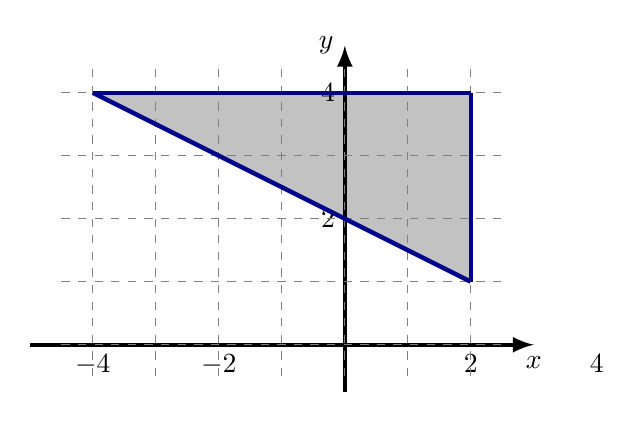
\begin{tikzpicture}[scale=0.8]
        \draw[fill=gray!80!black, opacity=0.4] (-4,4) -- (2,4) -- (2,1);        
        \draw[ultra thick,->,>=latex] (-5,0)--(3,0) node[below] {$x$};
        \draw[ultra thick,->,>=latex] (0,-0.75)--(0,4.75) node[left] {$y$};
        \draw (-4,0) node[below] {$-4$};          
        \draw (-2,0) node[below] {$-2$};          
        \draw (2,0) node[below] {$2$};          
        \draw (4,0) node[below] {$4$};          
        \draw (0,2) node[left] {$2$};        
        \draw (0,4) node[left] {$4$};
        \draw[help lines,gray,thin,dashed] (-4.5, -0.5) grid (2.5, 4.5);
        \draw[domain=-4:2,ultra thick,DarkBlue,samples=200] plot ({\x},{2-0.5*\x });
        \draw[domain=-4:2,ultra thick,DarkBlue,samples=200] plot ({\x},{4});
        \draw[ultra thick,-,DarkBlue,>=latex] (2,1)--(2,4);
    \end{tikzpicture}
    \end{center}     
    The area of the region is half the area of the rectangle whose width is 6 and height is 3. 
    $$\text{area of triangular region} = \frac12 ( 6 \cdot 3) = 9$$
    The region is bounded on the \textbf{left} by $y=2-x/2$, or $x=4-2y$. The region is also bounded on the \textbf{right} by $x=2$, and on the \textbf{top} by $y=4$. The region is 
    $$R = \{(x,y) \in \mathbb R^2 \, | \, 1\le y \le 4, \ 4-2y < x < 2\}$$
    Therefore, 
    \begin{align}
        a & = 1 \\
        b &= 4 \\
        c &= 4 - 2y \\
        d &= 2 \\
        g &= \frac{f(x,y)}{\text{area of region}} = \frac{16x+20y}{9} 
    \end{align}
    }
   \else

   \fi
\fi 





% UPWARDS PARABOLA AND A LINE
\ifnum \Version=5
    \part The area of the region bounded by $y=x^2-4$ and $y=x+2$ is $\displaystyle  \int_a^b \int_c^d f(x,y) \, dy \, dx$,  where $a=\framebox{\strut\hspace{1cm}}$, $b=\framebox{\strut\hspace{1cm}}$, $c=\framebox{\strut\hspace{2cm}}$, $d=\framebox{\strut\hspace{2cm}}$, and $f(x,y) = \framebox{\strut\hspace{2cm}}$.
    
    \ifnum \Solutions=1 
    {\color{DarkBlue} We want to determine where the two curves intersect. Setting them equal to each other: 
    \begin{align}
        x^2-4 &= x+2 \\
        0 &= x^2 - x - 6 \\
        0 &= (x-3)(x+2) \\
        x &= 3, -2
    \end{align}
    To obtain the $y-$coordinates, we can use either curve. Substituting the two $y-$values into either curve gives us two intersection points
    $$(-2,0), (3,5)$$
    It can help to sketch the two curves, as shown in the diagram below. 

    \begin{center}  
    \begin{tikzpicture}[scale=0.95]
        \begin{axis}[
        axis lines = middle, very thick,
        xlabel = {$x$},
        ylabel = {$y$},
        xmin=-3.5, xmax=6.75,
        ymin=-5, ymax=7.5,
        xtick={-2,-1,...,4,5},
        xticklabels={-2,-1,0,1,2,3,4,5},  
        ytick={-4,-2,...,6},
        yticklabels={-4,-2,0,2,4,6},
        ymajorgrids=true,
        xmajorgrids=true,
        grid style=dashed        
        ]
        % Plot 1
        \addplot [name path = A,
        -,
        domain = -3:3.25, ultra thick,DarkBlue,
        samples = 42] {x^2-4} 
        node [very near end, right] {$y=x^2-4$};
        \addplot [name path = B,
        -,
        domain = -3:4.25, ultra thick,DarkBlue,
        samples = 4] {x+2} 
        node [very near end, right=4pt] {$y=x+2$}; 
        % Fill area between paths
        \addplot [black!30, opacity=0.2] fill between [of = A and B, soft clip={domain=-2:3}];
        \end{axis}
    \end{tikzpicture}    
    \end{center}
    
    The region is bounded on the \textbf{bottom} by $y=x^2-4$, and bounded on the \textbf{top} by $y=x+2$. The region is 
    $$R = \{(x,y) \in \mathbb R^2 \, | \, -2 \le x \le 3, \quad x^2-4 < y < x+2 \}$$
    Therefore, 
    \begin{align}
        a & = -2 \\
        b &= +3 \\
        c &= x^2-4 \\
        d &= x+2 \\
        f &= 1
    \end{align}
    }
   \else

   \fi
\fi 





% SIDEWAYS PARABOLA AND A LINE 
\ifnum \Version=6
    \part The area of the region bounded by $x=1-y^2$ and $x=y-5$ is $\displaystyle  \int_a^b \int_c^d f(x,y) \, dx \, dy$,  where $a=\framebox{\strut\hspace{1cm}}$, $b=\framebox{\strut\hspace{1cm}}$, $c=\framebox{\strut\hspace{2cm}}$, $d=\framebox{\strut\hspace{2cm}}$, and $f(x,y) = \framebox{\strut\hspace{2cm}}$.
        
    \ifnum \Solutions=1 
    {\color{DarkBlue} We want to determine where the two curves intersect. Setting them equal to each other: 
    \begin{align}
        1-y^2 &= y - 5 \\
        0 &= y^2 + y - 6 \\
        0 &= (y+3)(y-2) \\
        y &= -3, 2
    \end{align}
    To obtain the $x-$coordinates, we can use either curve. Substituting the two $y-$values into either curve gives us two intersection points
    $$(-8,-3) \ \text{and} \ (-3,2)$$
    It can help to sketch the two curves, as shown in the diagram below. 
       \begin{center}     
    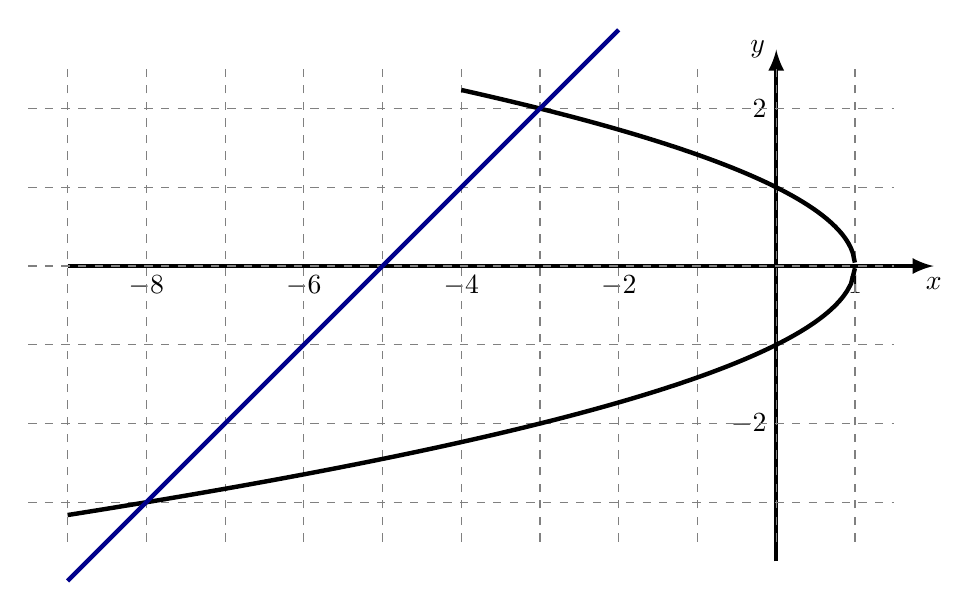
\begin{tikzpicture}[scale=1.0]
      \draw[ultra thick,->,>=latex] (-9,0)--(2,0) node[below] {$x$};
      \draw[ultra thick,->,>=latex] (0,-3.75)--(0,2.75) node[left] {$y$};
      \draw (-2,0) node[below] {$-2$};          
      \draw (-4,0) node[below] {$-4$};          
      \draw (-6,0) node[below] {$-6$};          
      \draw (-8,0) node[below] {$-8$};          
      \draw (1,0) node[below] {$1$};
      \draw (0,2) node[left] {$2$};        
      \draw (0,-2) node[left] {$-2$};
      \draw[help lines,gray,thin,dashed] (-9.5, -3.5) grid (1.5, 2.5);
      \draw[domain=-4:1,ultra thick,samples=200] plot ({\x},{sqrt(1-\x )});
      \draw[domain=-9:1,ultra thick,samples=200] plot ({\x},{-sqrt(1-\x )});
      \draw[domain=-9:-2,ultra thick,DarkBlue,samples=200] plot ({\x},{\x+5});
    \end{tikzpicture}
    \end{center}     
    The region is bounded on the \textbf{right} by $x=1-y^2$, and bounded on the \textbf{left} by $x=y-5$. The region is 
    $$R = \{(x,y) \in \mathbb R^2 \, | \, -3\le y \le 2, \quad y-5 < x < 1-y^2\}$$
    Therefore, 
    \begin{align}
        a & = -3 \\
        b &= +2 \\
        c &= y - 5 \\
        d &= 1-y^2 \\
        f &= 1
    \end{align}
    }
   \else

   \fi
\fi 








% SIDEWAYS PARABOLA AND A LINE 
\ifnum \Version=7
    \part The area of the region bounded by $x=1-y^2$ and $x=y-1$ is $\displaystyle  \int_a^b \int_c^d f(x,y) \, dx \, dy$,  where $a=\framebox{\strut\hspace{1cm}}$, $b=\framebox{\strut\hspace{1cm}}$, $c=\framebox{\strut\hspace{2cm}}$, $d=\framebox{\strut\hspace{2cm}}$, and $f(x,y) = \framebox{\strut\hspace{2cm}}$.
        
    \ifnum \Solutions=1 
    {\color{DarkBlue} We want to determine where the two curves intersect. Setting them equal to each other: 
    \begin{align}
        1-y^2 &= y - 1 \\
        0 &= y^2 + y - 2 \\
        0 &= (y+2)(y-1) \\
        y &= -2, 1
    \end{align}
    To obtain the $x-$coordinates, we can use either curve. Substituting the two $y-$values into either curve gives us two intersection points
    $$(-3,-2) \ \text{and} \ (0,1)$$
    It can help to sketch the two curves, as shown in the diagram below. 
       \begin{center}     
    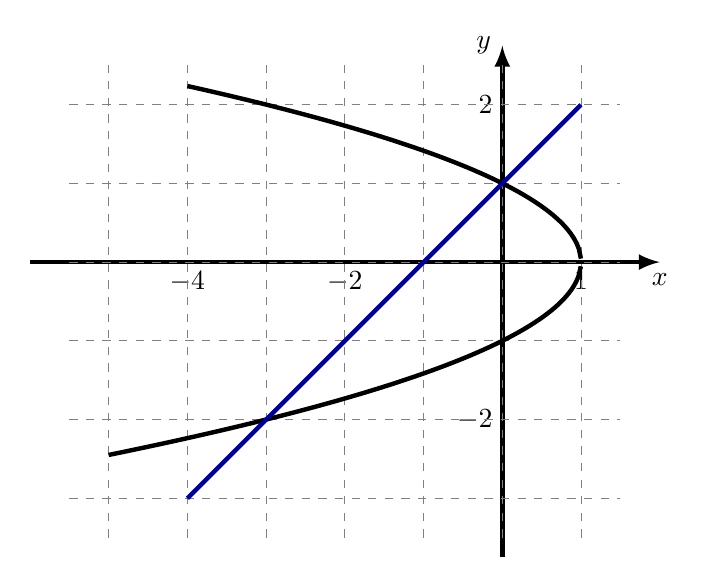
\begin{tikzpicture}[scale=1.0]
      \draw[ultra thick,->,>=latex] (-6,0)--(2,0) node[below] {$x$};
      \draw[ultra thick,->,>=latex] (0,-3.75)--(0,2.75) node[left] {$y$};
      \draw (-2,0) node[below] {$-2$};          
      \draw (-4,0) node[below] {$-4$};          
      \draw (1,0) node[below] {$1$};
      \draw (0,2) node[left] {$2$};        
      \draw (0,-2) node[left] {$-2$};
      \draw[help lines,gray,thin,dashed] (-5.5, -3.5) grid (1.5, 2.5);
      \draw[domain=-4:1,ultra thick,samples=200] plot ({\x},{sqrt(1-\x )});
      \draw[domain=-5:1,ultra thick,samples=200] plot ({\x},{-sqrt(1-\x )});
      \draw[domain=-4:1,ultra thick,DarkBlue,samples=200] plot ({\x},{\x+1});
    \end{tikzpicture}
    \end{center}     
    The region is bounded on the \textbf{right} by $x=1-y^2$, and bounded on the \textbf{left} by $x=y-1$. The region is 
    $$R = \{(x,y) \in \mathbb R^2 \, | \, -2\le y \le 1, \quad y-1 < x < 1-y^2\}$$
    Therefore, 
    \begin{align}
        a & = -2 \\
        b &= +1 \\
        c &= y - 1 \\
        d &= 1-y^2 \\
        f &= 1
    \end{align}
    }
   \else

   \fi
\fi 




\ifnum \Version=8
    \part The average value of $f(x,y) = 8x-4y^2$ over the region in the first quadrant bounded by $x=2$, $y=4$, and $y=4-2x$ is $\displaystyle  \int_a^b \int_c^d g(x,y) \, dx \, dy$,  where $a=\framebox{\strut\hspace{1cm}}$, $b=\framebox{\strut\hspace{1cm}}$, $c=\framebox{\strut\hspace{2cm}}$, $d=\framebox{\strut\hspace{2cm}}$, and $g(x,y) = \framebox{\strut\hspace{2cm}}$.

    \ifnum \Solutions=1 
    {\color{DarkBlue} 
    The average value of a function $f(x,y)$ over a region $R$ is given by 
    \begin{align}
        \text{Average value of }f\text{ over region }R &= \frac{1}{\text{area of region }R}\iint_R f \, dA \\&= \iint_R \frac{f(x,y)}{\text{area of region }R} \, dA
    \end{align}
    Therefore to obtain $g(x,y)$ we can calculate
    \begin{align}
        g(x,y) = \frac{f(x,y)}{\text{area of region }R}
    \end{align}
    So we need the area of the region. It can help to sketch the region, as shown in the diagram below. 
       \begin{center}     
        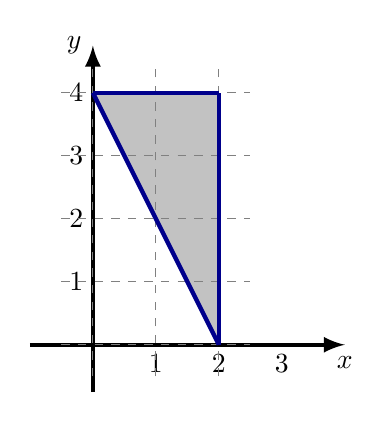
\begin{tikzpicture}[scale=0.8]
        \draw[fill=gray!80!black, opacity=0.4] (2,0) -- (2,4) -- (0,4);        
        \draw[ultra thick,->,>=latex] (-1,0)--(4,0) node[below] {$x$};
        \draw[ultra thick,->,>=latex] (0,-0.75)--(0,4.75) node[left] {$y$};
        \draw (1,0) node[below] {$1$};          
        \draw (2,0) node[below] {$2$};          
        \draw (3,0) node[below] {$3$};          
        \draw (0,1) node[left] {$1$};        
        \draw (0,2) node[left] {$2$};
        \draw (0,3) node[left] {$3$};
        \draw (0,4) node[left] {$4$};
        \draw[help lines,gray,thin,dashed] (-0.5, -0.5) grid (2.5, 4.5);
        \draw[domain=0:2,ultra thick,DarkBlue,samples=200] plot ({\x},{4-2*\x });
        \draw[domain=0:2,ultra thick,DarkBlue,samples=200] plot ({\x},{4 });
        \draw[ultra thick,-,DarkBlue,>=latex] (2,0)--(2,4);
    \end{tikzpicture}
    \end{center}     
    The region is bounded on the \textbf{right} by $y=4-2x$, or $x=2-y/2$. The region is also bounded on the \textbf{left} by $x=0$. The region is 
    $$R = \{(x,y) \in \mathbb R^2 \, | \, 0\le y \le 4, \ 0 < x < 2-y/2\}$$
    The area of the region is half the area of the rectangle whose length is 2 and height is 4. 
    $$\text{area of triangular region} = \frac12 ( 2 \cdot 4) = 4$$    
    Therefore, 
    \begin{align}
        a & = 0 \\
        b &= 4 \\
        c &= 2-y/2 \\
        d &= 2 \\
        g &= \frac{8x-4y^2}{4} = 2x - y^2
    \end{align}
    }
   \else

   \fi
\fi 



% DOWNWARDS PARABOLA AND A LINEAR
\ifnum \Version=9
    \part The area of the region bounded by $y=1-x^2$ and $y=x-1$ is $\displaystyle  \int_a^b \int_c^d f(x,y) \, dy \, dx$,  where $a=\framebox{\strut\hspace{1cm}}$, $b=\framebox{\strut\hspace{1cm}}$, $c=\framebox{\strut\hspace{2cm}}$, $d=\framebox{\strut\hspace{2cm}}$, and $f(x,y) = \framebox{\strut\hspace{2cm}}$.
    
    \ifnum \Solutions=1 
    {\color{DarkBlue} We want to determine where the two curves intersect. Setting them equal to each other: 
    \begin{align}
        1-x^2 &= x - 1 \\
        0 &= x^2 + x - 2 \\
        0 &= (x+2)(x-1) \\
        x &= -2, 1
    \end{align}
    To obtain the $y-$coordinates, we can use either curve. Substituting the two $x-$values into either curve gives us two intersection points
    $$(-2,-3), (1,0)$$
    It can help to sketch the two curves, as shown in the diagram below. 
       \begin{center}     
    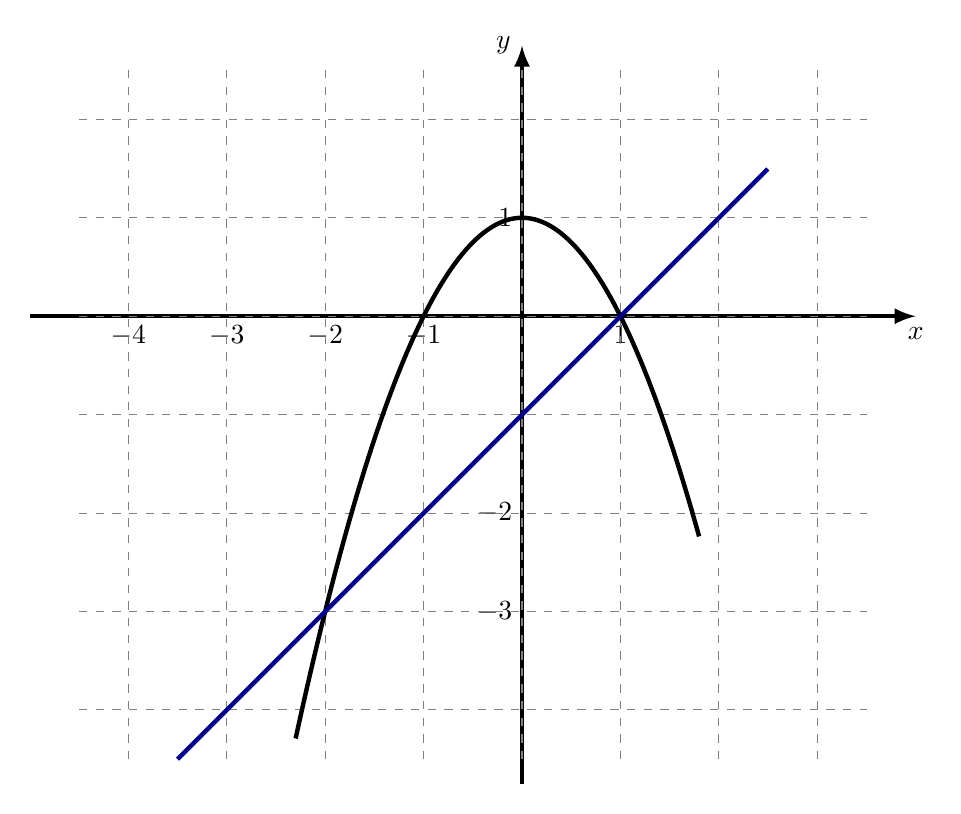
\begin{tikzpicture}[scale=1.25]
      \draw[ultra thick,->,>=latex] (-5,0)--(4,0) node[below] {$x$};
      \draw[ultra thick,->,>=latex] (0,-4.75)--(0,2.75) node[left] {$y$};
      \draw (-1,0) node[below] {$-1$};          
      \draw (-2,0) node[below] {$-2$};          
      \draw (-3,0) node[below] {$-3$};          
      \draw (-4,0) node[below] {$-4$};          
      \draw (1,0) node[below] {$1$};
      \draw (0,1) node[left] {$1$};        
      \draw (0,-2) node[left] {$-2$};
      \draw (0,-3) node[left] {$-3$};
      \draw[help lines,gray,thin,dashed] (-4.5, -4.5) grid (3.5, 2.5);
      \draw[domain=-2.3:1.8,ultra thick,samples=200] plot ({\x},{1-\x*\x});
      \draw[domain=-3.5:2.5,ultra thick,DarkBlue,samples=200] plot ({\x},{\x-1});
    \end{tikzpicture}
    \end{center}     
    The region is bounded on the \textbf{right} by $x=-y^2$, and bounded on the \textbf{left} by $x=y-2$. The region is 
    $$R = \{(x,y) \in \mathbb R^2 \, | \, -2\le x \le 1, \quad x-1 < y < 1-x^2\}$$
    Therefore, 
    \begin{align}
        a & = -2 \\
        b &= +1 \\
        c &= x -1 \\
        d &= 1-x^2 \\
        f &= 1
    \end{align}
    }
   \else

   \fi
\fi 
